\documentclass{article}
\usepackage[utf8]{inputenc}
\usepackage{titling}
\usepackage{graphicx}
\usepackage{xcolor}
\usepackage[colorlinks=true,linkcolor=darkgray, urlcolor =gray]{hyperref}
\usepackage[spanish]{babel}
\DeclareUnicodeCharacter{301}{~}
\newcommand\tab[1][1cm]{\hspace*{#1}}
\usepackage{url}


\begin{titlepage}
  \vspace*{4cm}  {\fontsize{28}{34}\selectfont\bfseries Tarea 3: aplicación completa}
  \hfill
  \begin{center}

\includegraphics[scale=0.8]{images/icon.jpg}
\end{center}
  {\large Simón Vallejo\\Sofía Merino\\Raúl Requena\\Cristina Díaz\\Alejandro Aguayo \hfill}
  \date{}
\end{titlepage}

\renewcommand\maketitlehooka{\null\mbox{}\vfill}
\renewcommand\maketitlehookd{\vfill\null}


\begin{document}

\addcontentsline{toc}{section}{Índice general}

\begin{titlingpage}
\maketitle
\end{titlingpage}

\newpage

\tableofcontents

\newpage

\section{Modificaciones a entregas anteriores}

\subsection{Entrega 1}

\textbf{Modelo Entidad-Relación}

\begin{center}
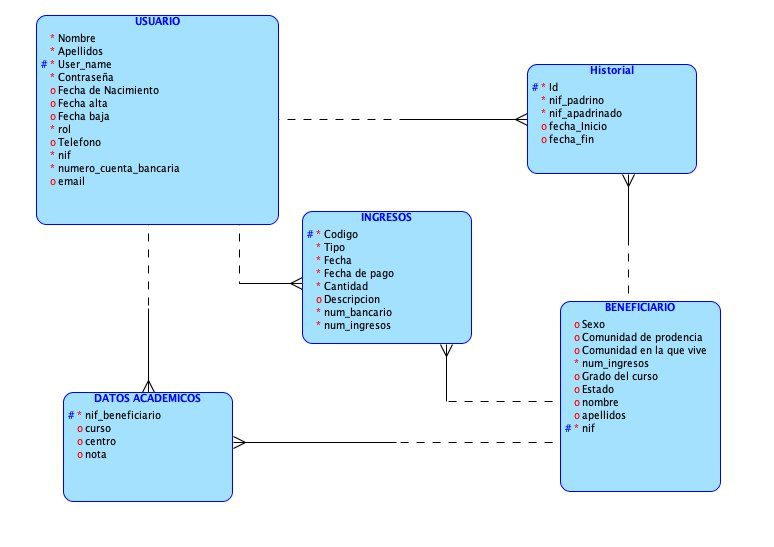
\includegraphics[scale=0.5]{images/entidades.jpg}
\end{center}

Este es el modelo entidad-relación de nuestra aplicación. Debido a que el anterior modelo contenía múltiples fallos, nos hemos visto obligados a modificarlo y este es el resultado.
Como vemos. Posee una entidad usuario con sus respectivos atributos y como clave primaria el nombre del usuario. Esta entidad está relacionada con las entidades Historial, ingresos y datos académicos. \\
Es muy importante el atributo rol de esta entidad ya que distingue entre socios y trabajadores. Por ejemplo, en el caso de la relación uno a muchos entre la entidad Usuario y la entidad Historial indica que un usuario puede tener muchos historiales pero un historial tiene que pertenecer a un solo usuario. Aquí, es donde el rol juega un papel muy importante, ya que en este caso solo tendrán historiales los que tengan el rol de socio.\\
El caso contrario para en el caso de los datos académicos, en el cual solo los trabajadores podrán añadir estos datos. La relación es uno a muchos ya que un trabajador podrá añadir varias notas a sus alumnos, pero una nota solo puede ser añadida por un trabajador y no por varios.\\
Con la entidad Datos Académicos lo que se pretende es almacenar las notas del curso de cada alumno. En nuestro caso, hemos utilizado una nota global de todo el curso para evaluarlo. Otra opción era añadir un atributo llamado asignatura que fuera clave compuesta con el nif del usuario. Esta opción es mejor que la que hemos elegido, pero por problemas a la hora de implementarlo hemos tenido que optar por esta opción.\\
La entidad Historial se aspira a conseguir gestionar los apadrinamientos de los niños. Como clave primaria una id para cada historial, esta entidad almacena los NIFs tanto de los socios como de los niños para tenerlos relacionados.\\
La entidad ingresos gestiona las donaciones por parte de los padrinos a los Niños. A cada ingreso se le asigna un código aleatorio que será la clave primaria, además se almacenaran los datos de las cuentas tanto del socio como del niño, así como, la cantidad, la fecha de realización y la fecha en la que se realizara el pago. La relación uno a muchos entre Usuario e Ingresos indica que los usuarios pueden realizar varios ingresos, pero no pueden realizar un único ingreso entre varios usuarios. Mientras que la relación Ingresos-Beneficiario muestra que los niños pueden recibir varios ingresos pero un ingreso no puede ir destinado a varios niños.\\
Para terminar, la clase Beneficiario cuenta con el nif como clave primaria y con num\_ingresos como atributo importante ya que almacena la cuenta en la que el niño recibirá el dinero.

Los cambios del modelo con respecto a la entrega anterior, han sido los siguientes: 

\begin{itemize}
\item Hemos añadido la entidad Usuario.
\item Hemos añadido las relaciones en las entidades JPA.
\item Modificación de la relación entre ingresos y socios para que un ingreso no pertenezca a varios socios.
\item Getters/Setters incluidos en las entidades.
\end{itemize}

Con respecto a los requisitos anteriormente entregados, estos son los que se han conseguido implementar:\\
RF 1: Creación, lectura de los datos de usuarios y beneficiarios.\\
RF 2: Registro y lectura de ingresos.\\
RF 3: Gestión de datos académicos: Inserción de datos y notas, así como, la lectura de los distintos datos del alumno.\\
RF 4: Gestión de historial de apadrinamiento: Inserción de datos de los apadrinamientos.\\

\newpage

\textbf{Java Persistance API (JPA)}

\begin{center}
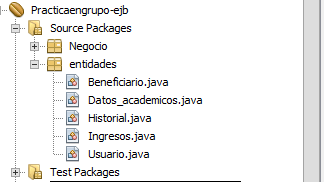
\includegraphics[scale=0.5]{images/tree.png}
\end{center}

En este apartado vamos a explicar todas las entidades creadas para la conexión de la base de datos.\\
Primero tenemos Beneficiario, clase que gestiona a los niños de la base de datos.

\begin{center}
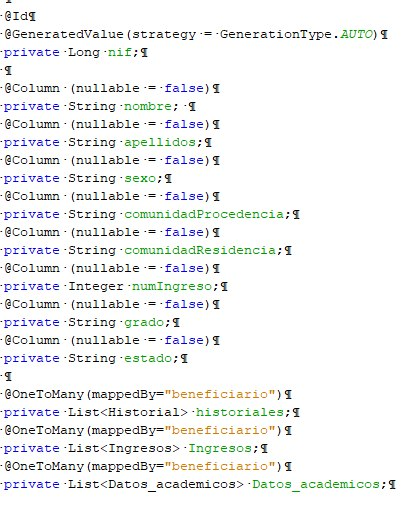
\includegraphics[scale=0.5]{images/beneficiario.jpg}
\end{center}

En ella se describen los distintos atributos que tiene los niños, mencionando que ninguno puede ser nulos al ser metidos en la base de datos y el Nif debe ser único.
Debajo de los atributos tenemos las relaciones de las distintas entidades en la base de datos, en este caso tiene relación uno a muchos con la entidad Historial, Ingresos y con Datos Académicos.\\
Los distintos get y set necesarios para cada atributo y sus propios métodos hashCode(),
equals() y toString().

\begin{center}
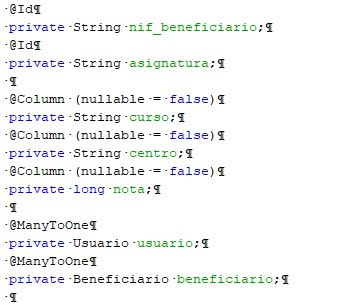
\includegraphics[scale=0.5]{images/relaciones.jpg}
\end{center}

Como segunda entidad tenemos Datos Académicos la cual es la encargada de guardar todos los datos relacionados con los estudios de los distintos niños.
Donde el nif del niño y la asignatura son únicos.
En cuanto a las relaciones con otras entidades tenemos una muchos a uno con Usuario y otra igual con beneficiario. 

\begin{center}
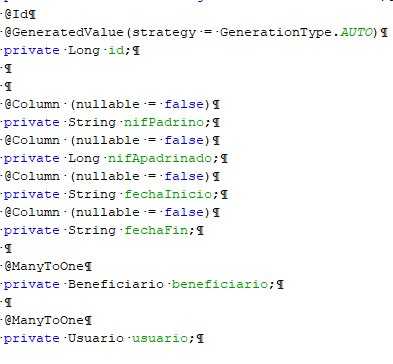
\includegraphics[scale=0.5]{images/historial.jpg}
\end{center}

La entidad Historial es una entidad intermedia entre las entidades Usuario y Beneficiario, la cual se utiliza para almacenar los niños apadrinados y sus padrinos.

\begin{center}
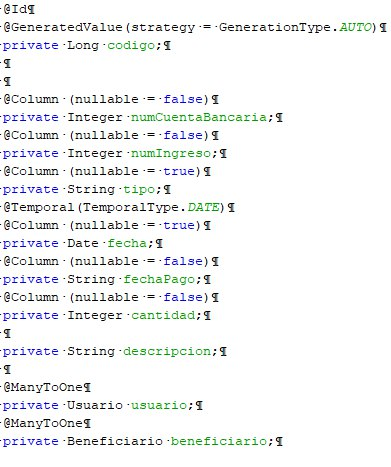
\includegraphics[scale=0.35]{images/ingresos.jpg}
\end{center}

Estos son los atributos de la entidad Ingresos y como se han generado sus distintas relaciones.

\begin{center}
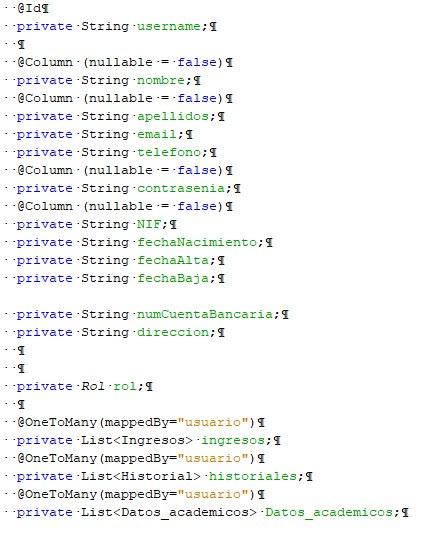
\includegraphics[scale=0.5]{images/usuarios.jpg}
\end{center}

Por último tenemos la entidad Usuario que gestiona los datos tanto de los socios como de los trabajadores de la asociación.
Mencionando que el Usuario es la clave principal y por tanto debe ser único.


\subsection{Entrega 2}

Las navegación entre las diferentes páginas es la siguiente:

\begin{center}
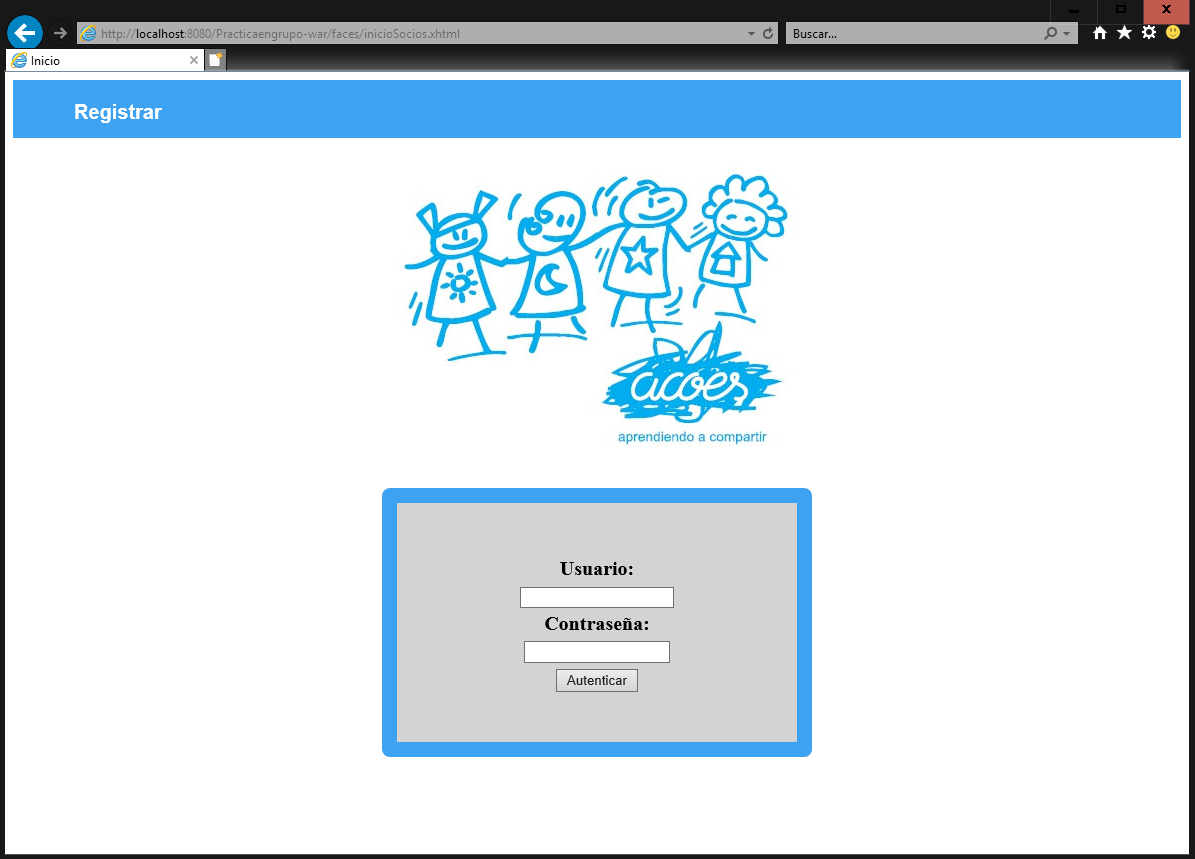
\includegraphics[scale=0.5]{capturas/INDEX.PNG}
\end{center}

Empezamos en el índex, pudiendo iniciar sesión o registrarnos.

\begin{center}
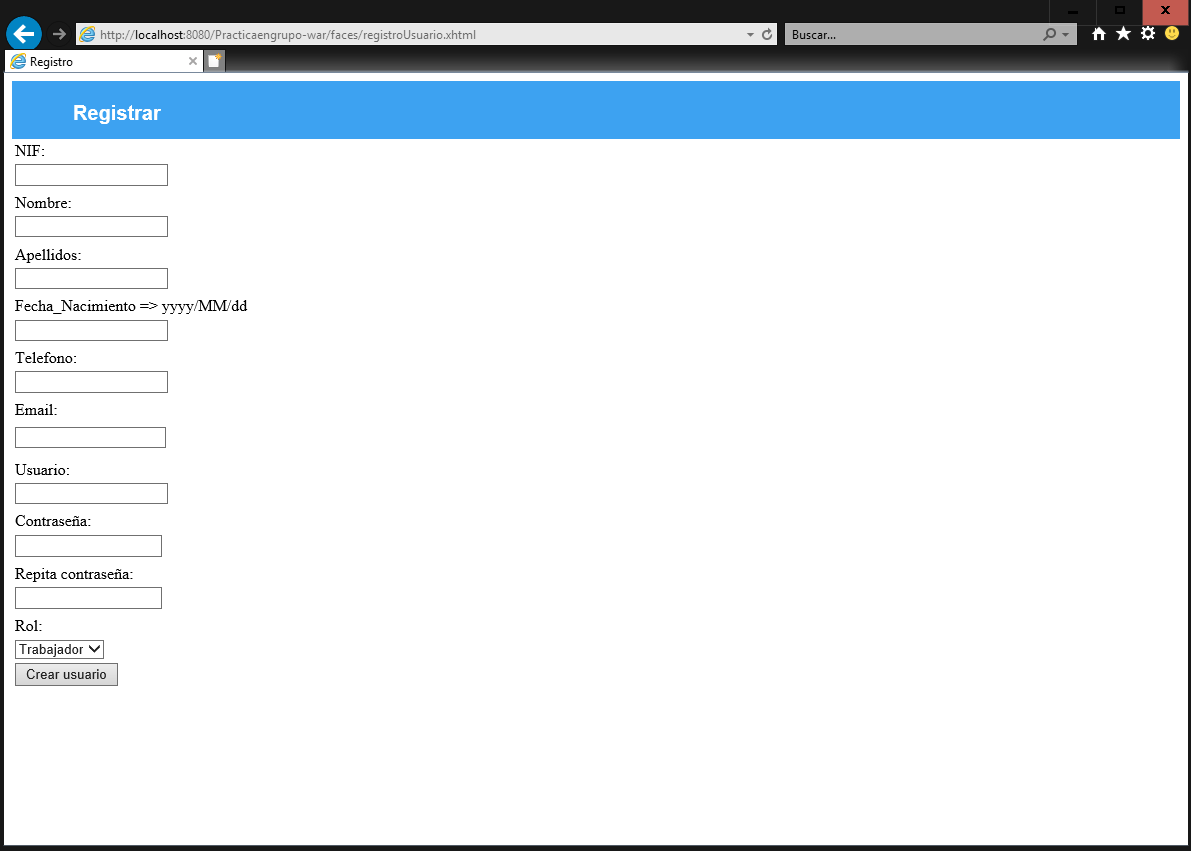
\includegraphics[scale=0.5]{capturas/REGISTRO.PNG}
\end{center}

Si al registrarnos, lo hacemos correctamente, podemos ver lo siguiente:

\begin{center}
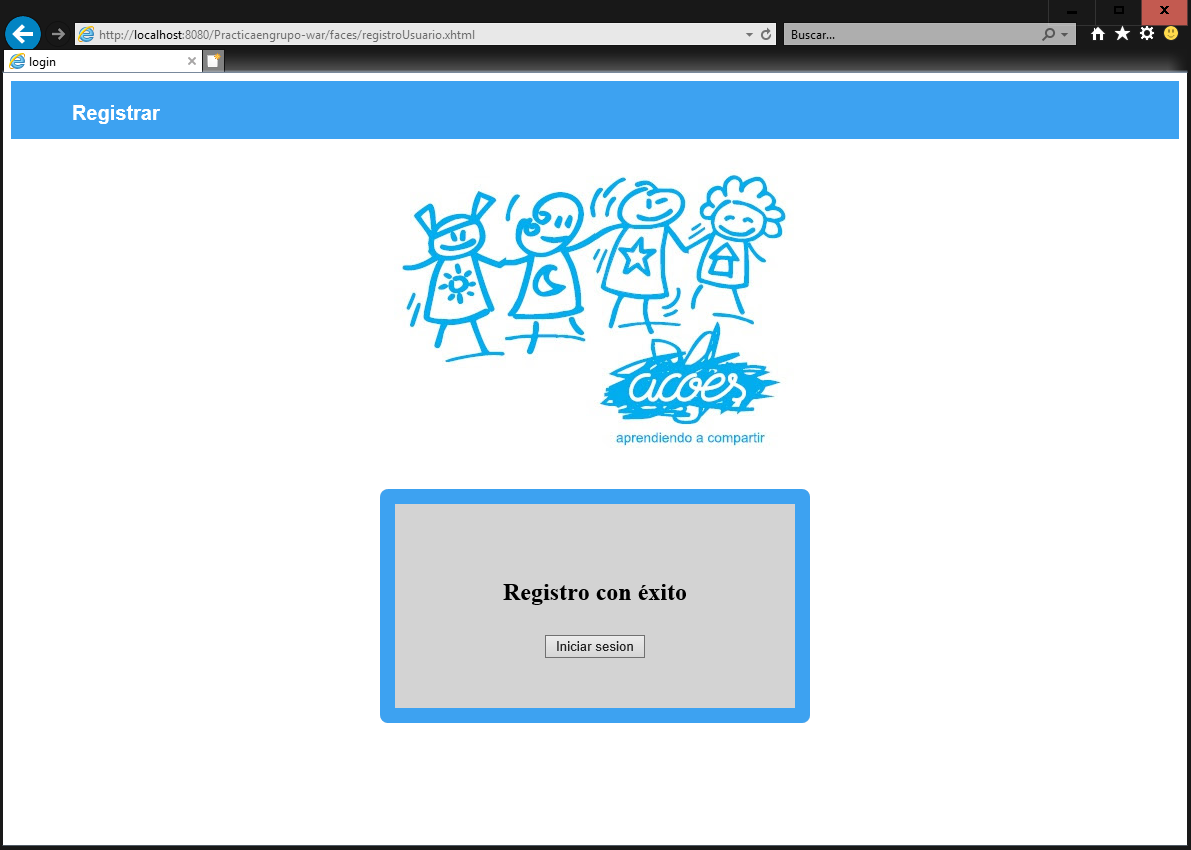
\includegraphics[scale=0.5]{capturas/REGISTROCONEXITO.PNG}
\end{center}

Si somos trabajadores, veremos esta pantalla:

\begin{center}
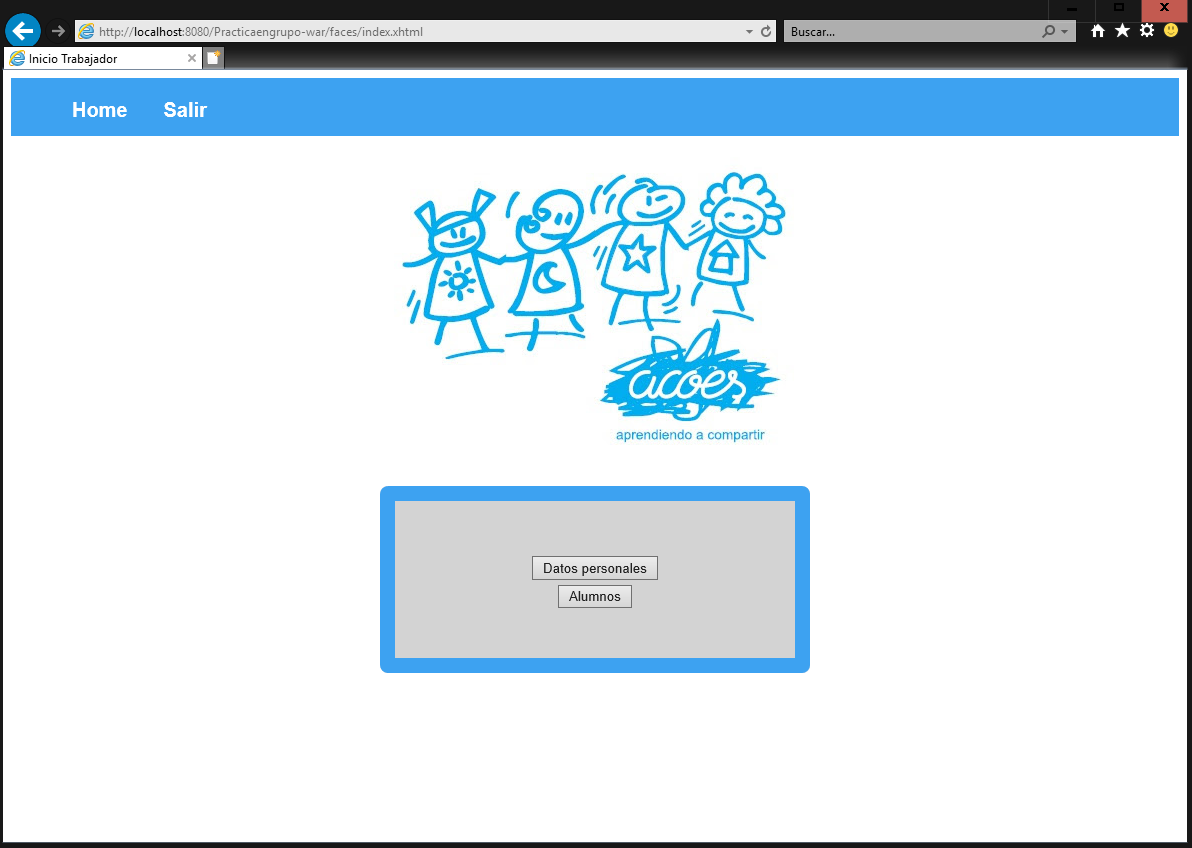
\includegraphics[scale=0.5]{capturas/INICIOTRABAJADORES.PNG}
\end{center}

Mientras que si somos socios, será:

\begin{center}
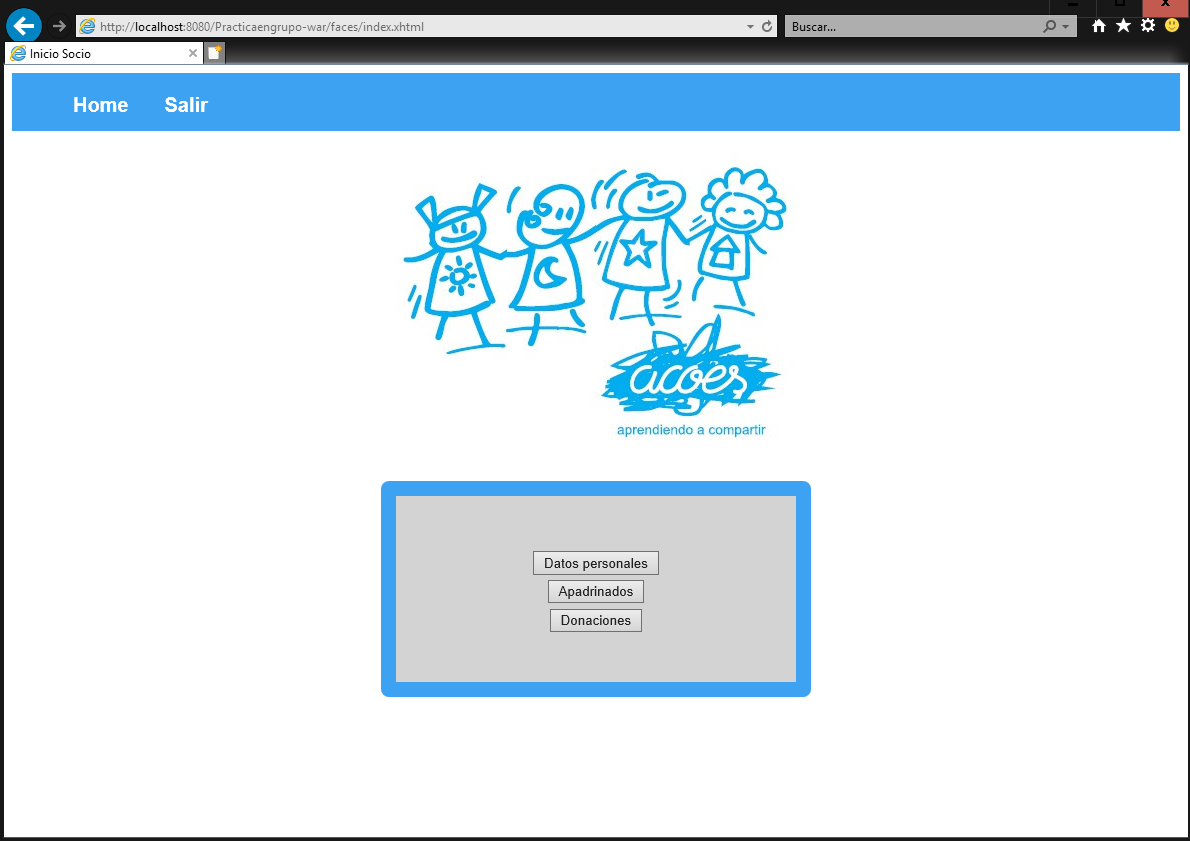
\includegraphics[scale=0.5]{capturas/INICIOSOCIOS.PNG}
\end{center}

Como trabajador, puedes añadir alumnos y sus calificaciones, y por supuesto, consultar la información respectiva a estos alumnos. 

\begin{center}
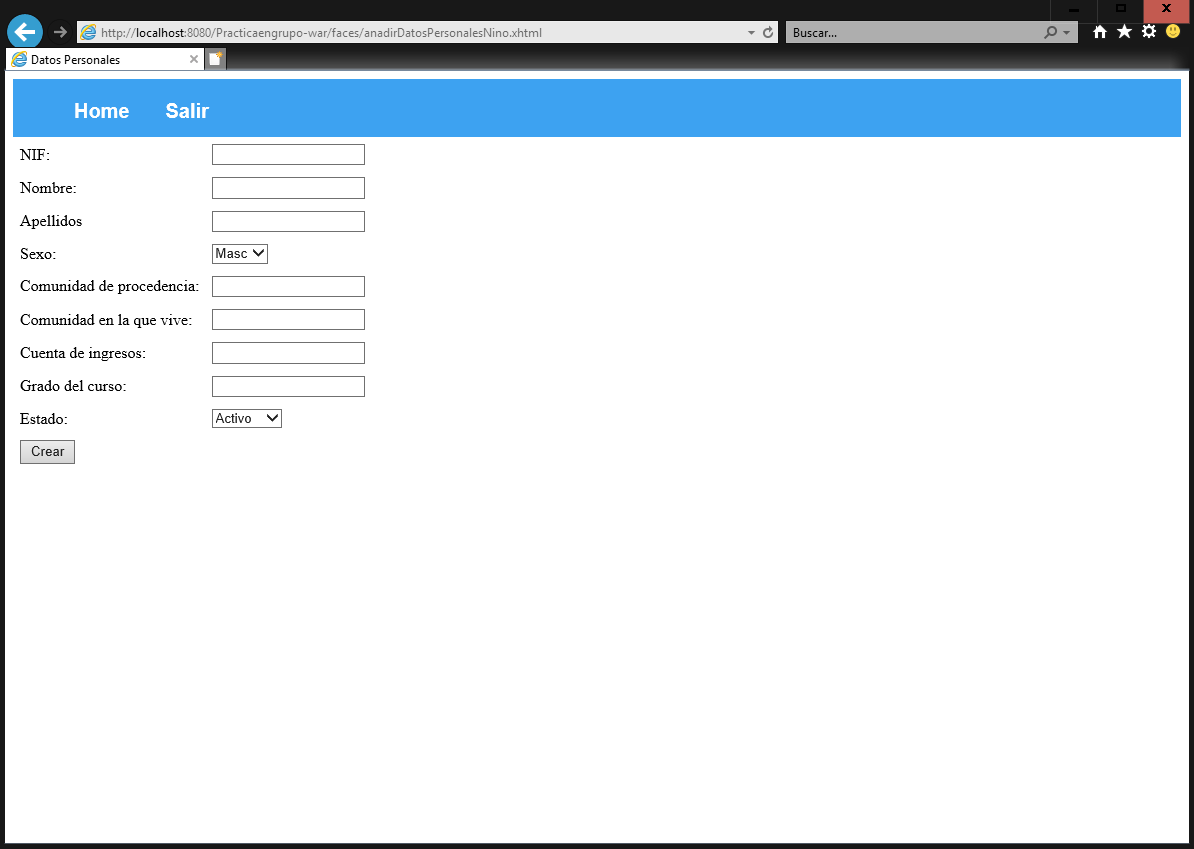
\includegraphics[scale=0.5]{capturas/ANADIRALUMNOS.PNG}
\end{center}

\begin{center}
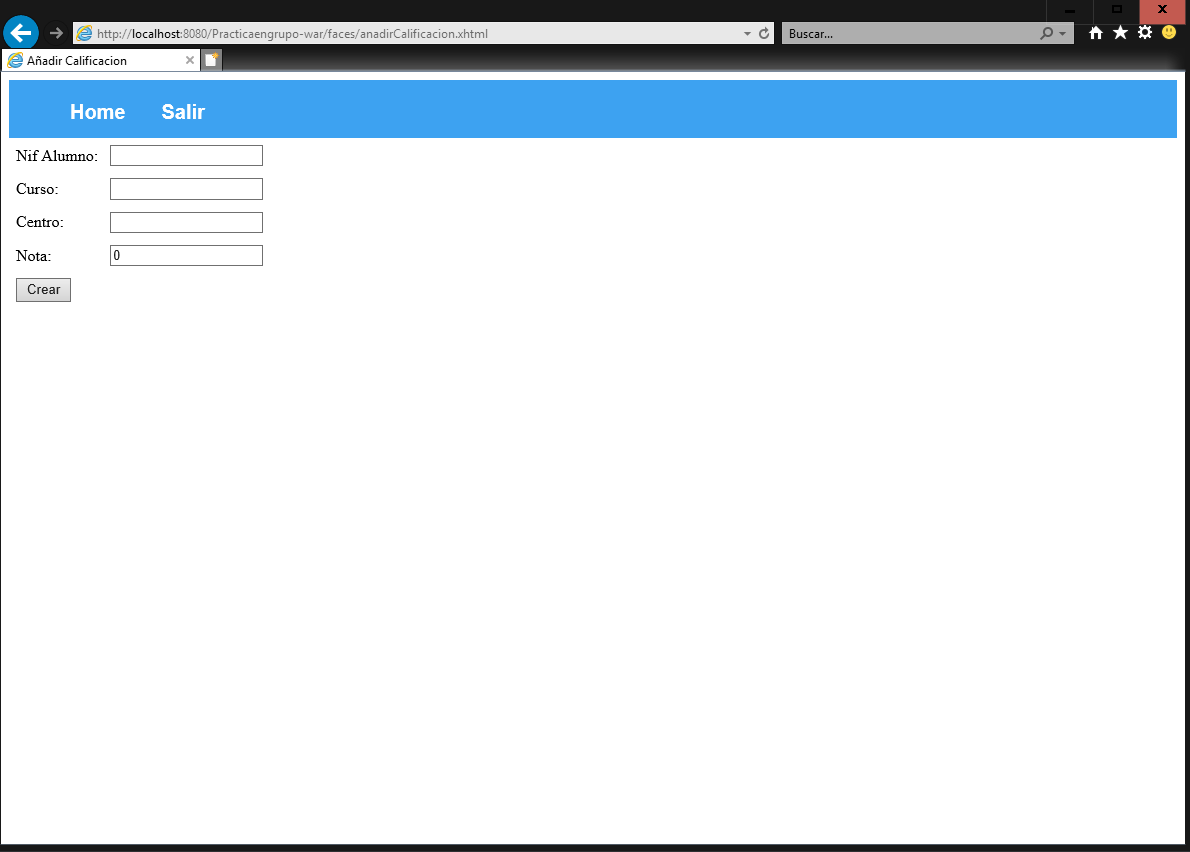
\includegraphics[scale=0.5]{capturas/ANADIRCALIFICACIONALUMNOS.PNG}
\end{center}

\begin{center}
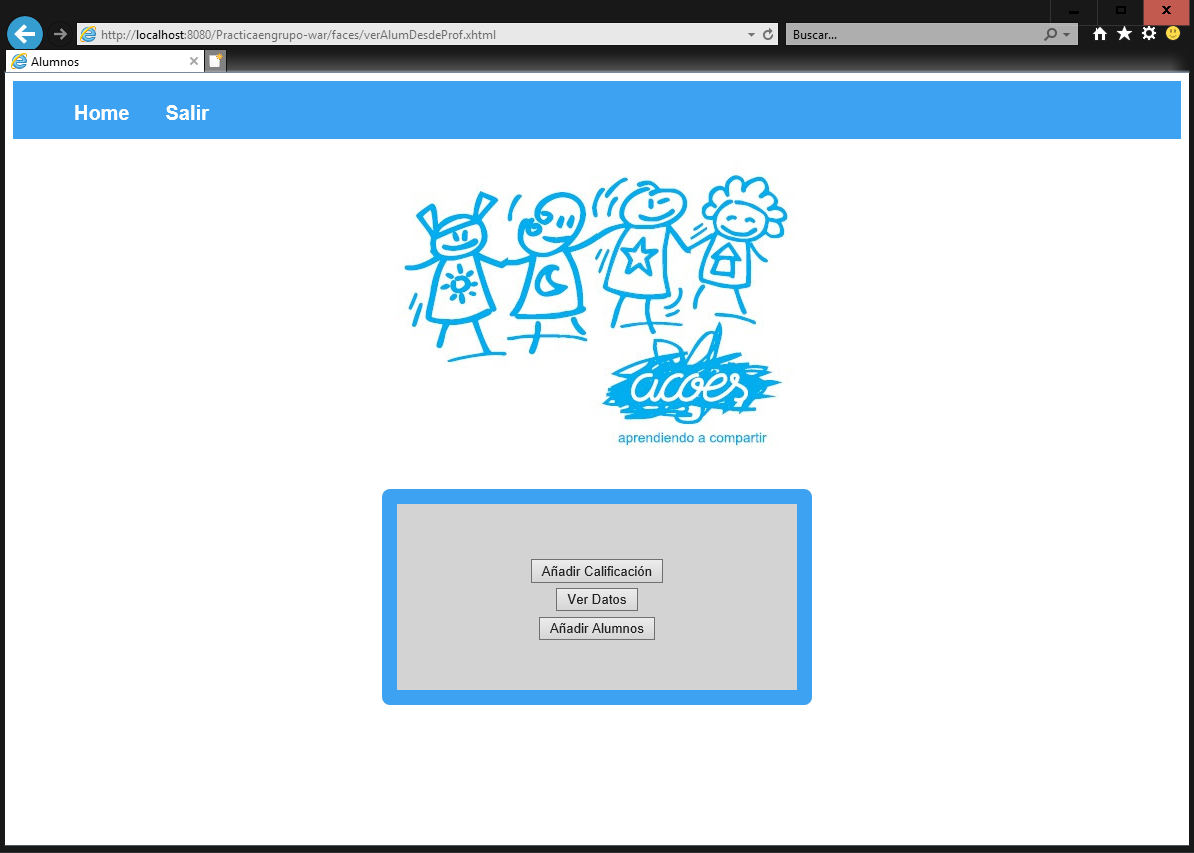
\includegraphics[scale=0.5]{capturas/COSASDELOSALUMNOS.PNG}
\end{center}

\begin{center}
\includegraphics[scale=0.5]{capturas/VERDATOSYCALIFICACIONESDESDETRABAJADORDELOSNINOS.PNG}
\end{center}

Como socio, puedes apadrinar, ver los datos de tus apadrinados y enviarles dinero:

\begin{center}
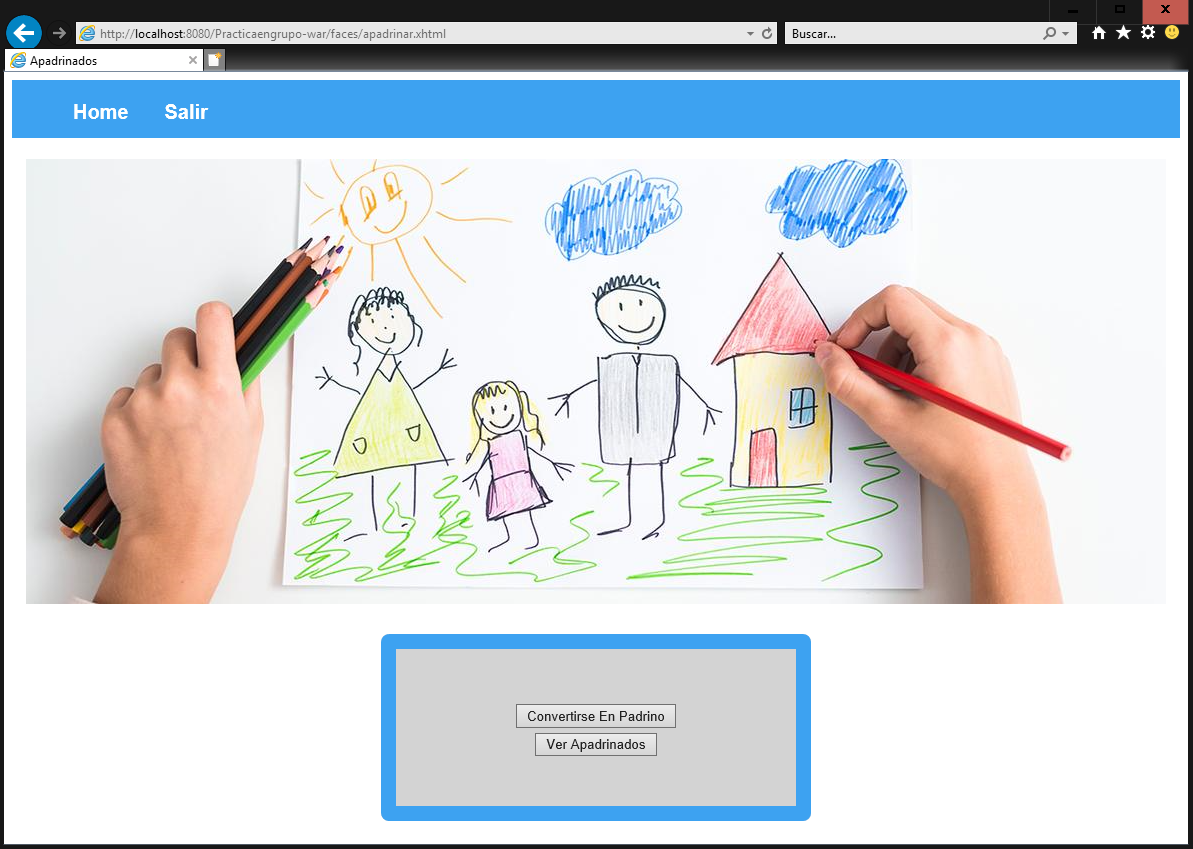
\includegraphics[scale=0.5]{capturas/APADRINADOS.PNG}
\end{center}

\begin{center}
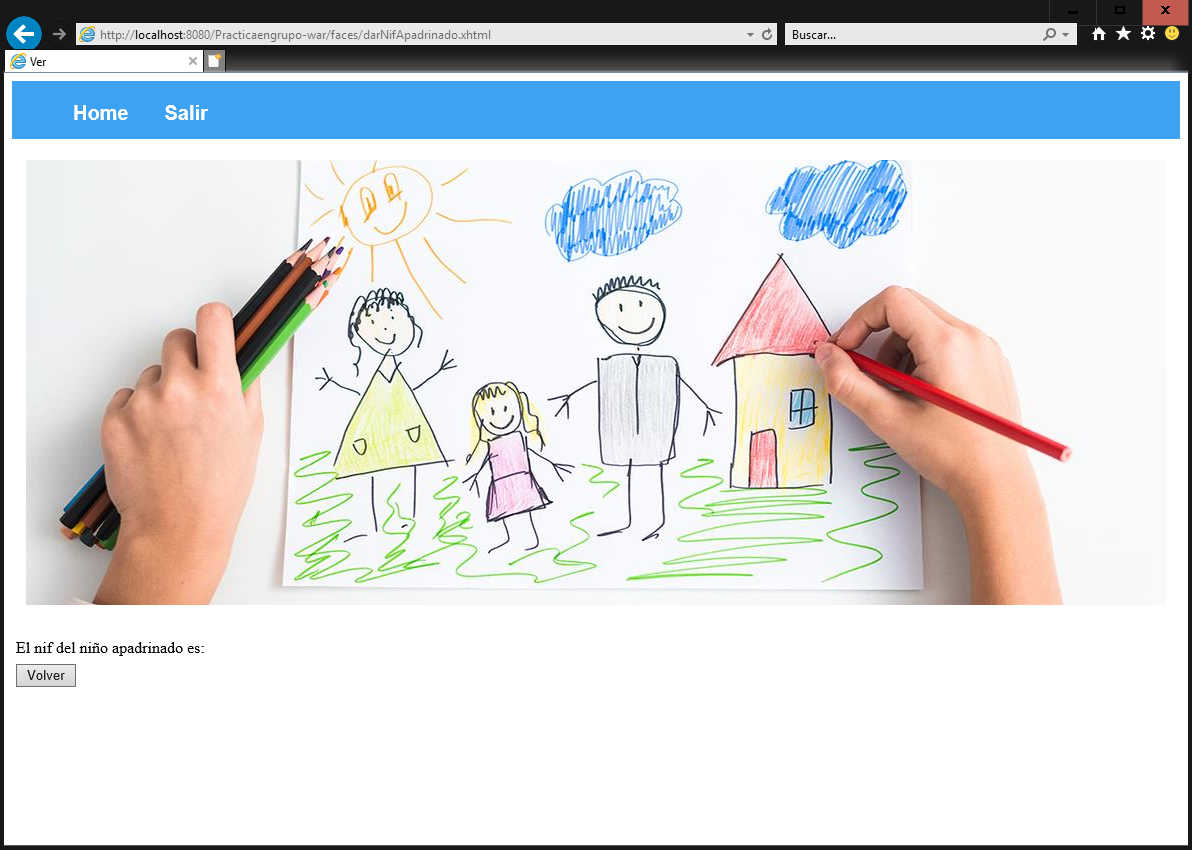
\includegraphics[scale=0.5]{capturas/NINOAPADRINADO.PNG}
\end{center}

\begin{center}
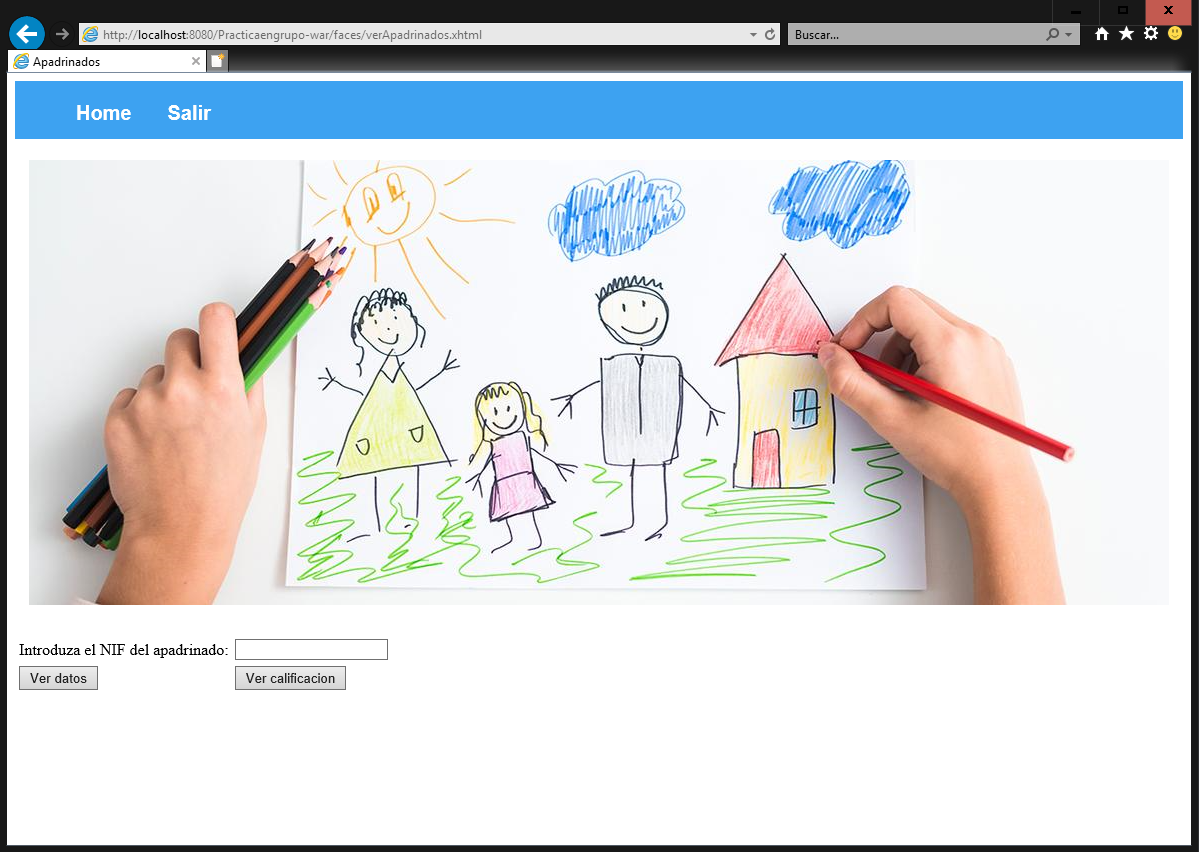
\includegraphics[scale=0.5]{capturas/VERAPADRINADOS.PNG}
\end{center}

\begin{center}
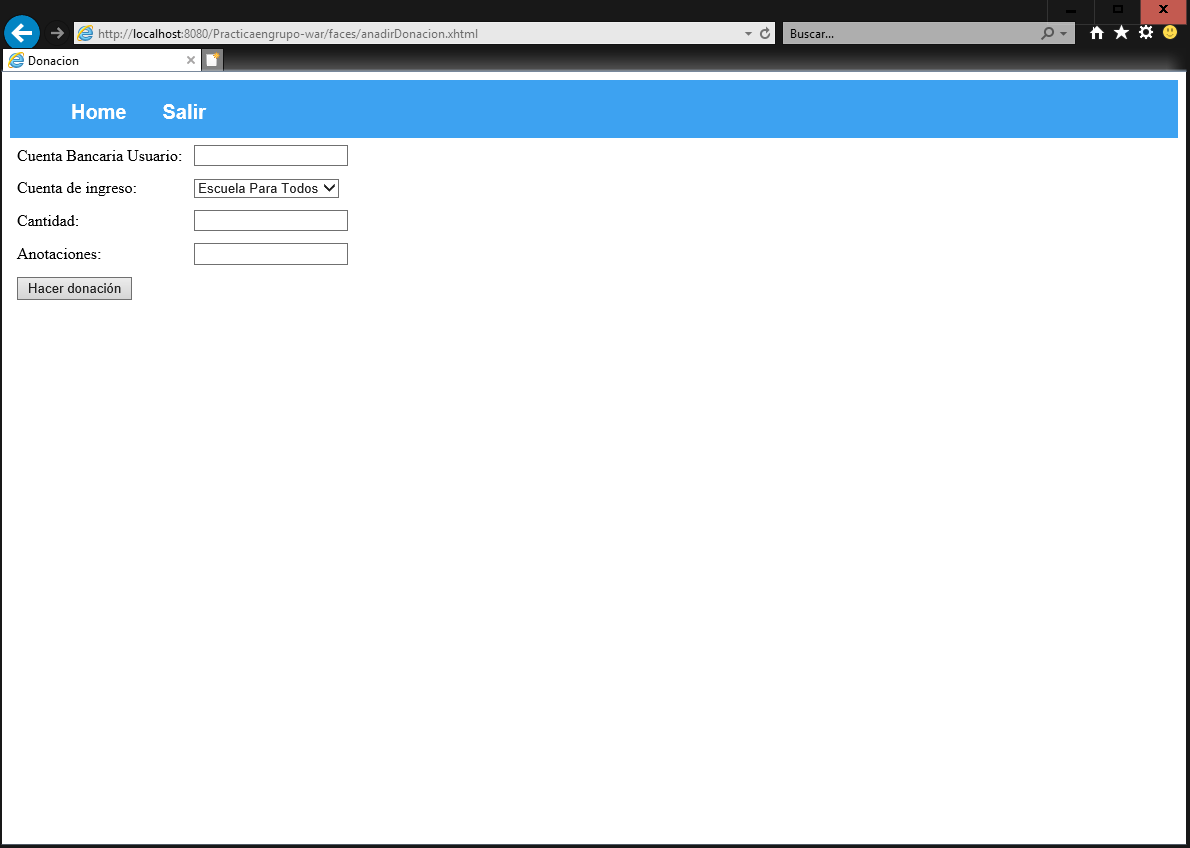
\includegraphics[scale=0.5]{capturas/ANADIRDONACION.PNG}
\end{center}

\begin{center}
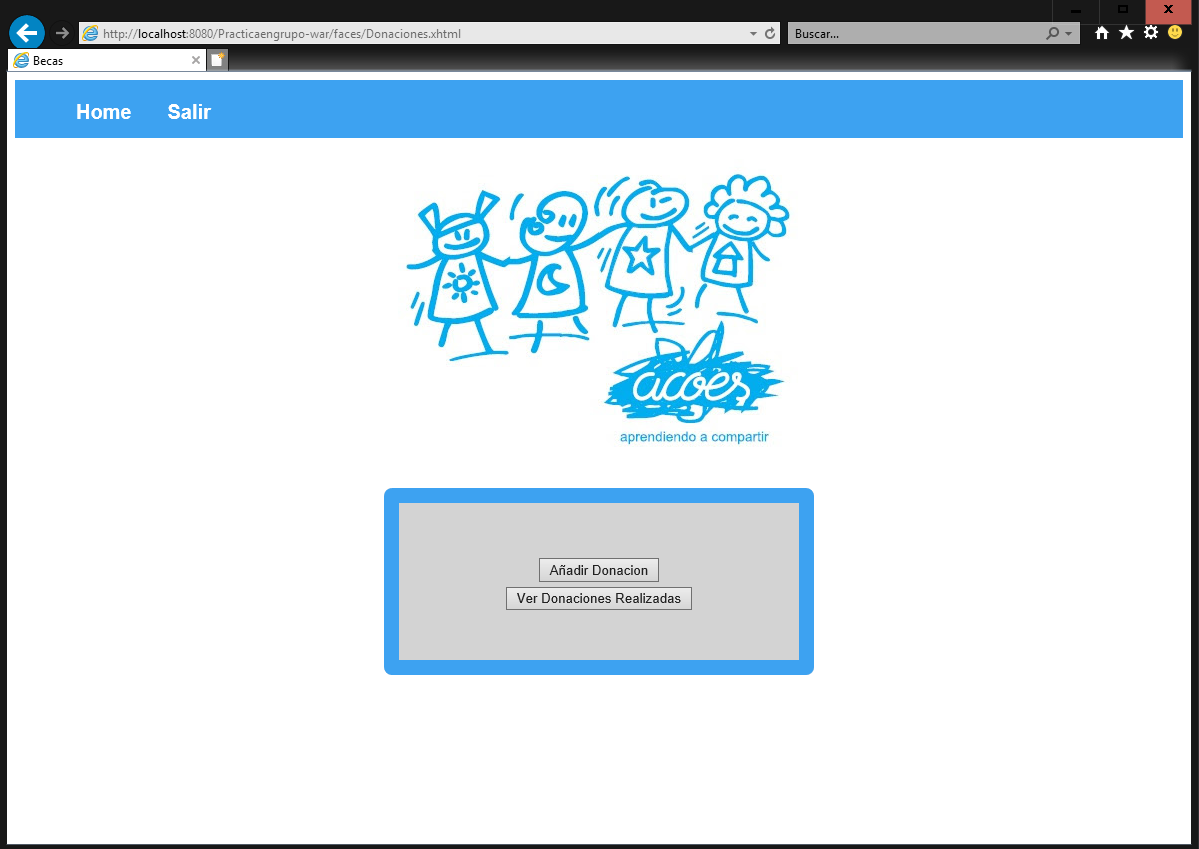
\includegraphics[scale=0.5]{capturas/DONACIONES.PNG}
\end{center}

Ambos pueden ver sus datos personales y modificarlos:

\begin{center}
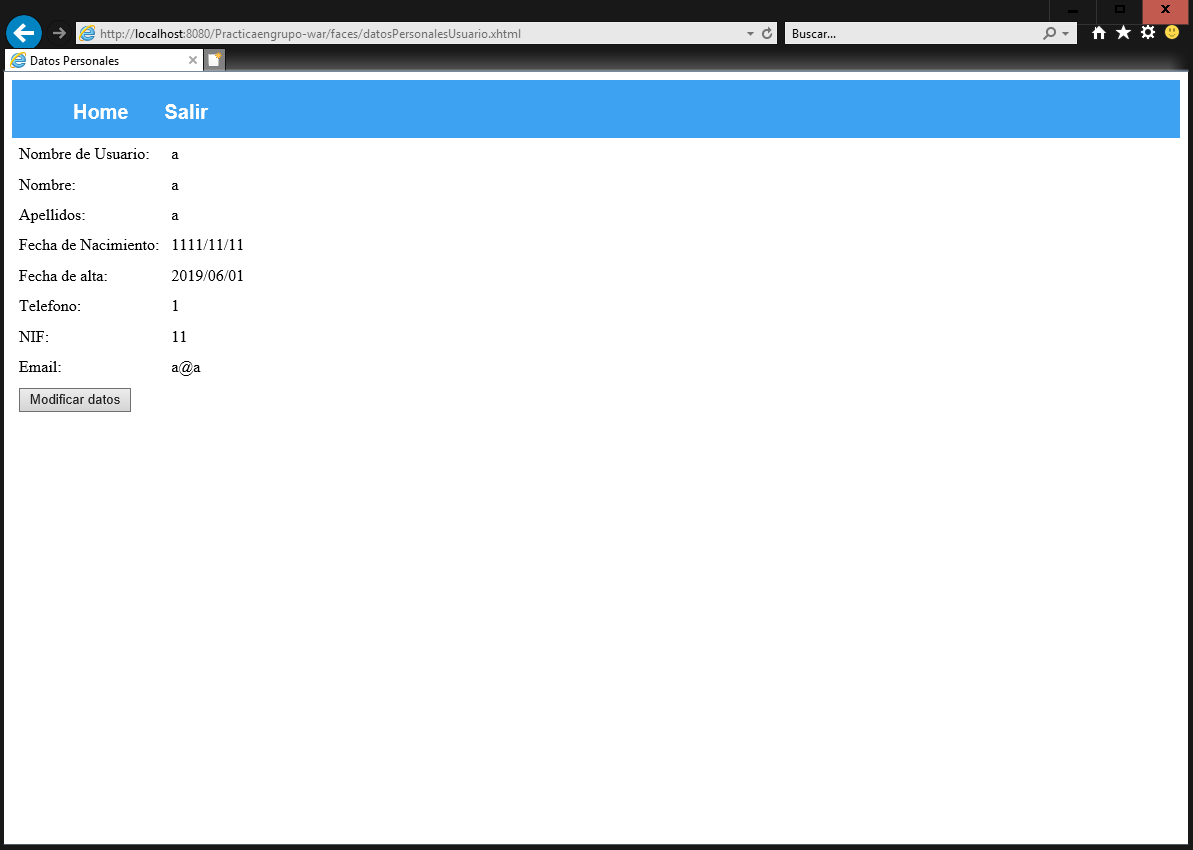
\includegraphics[scale=0.5]{capturas/VERDATOSPERSONALES.PNG}
\end{center}

\begin{center}
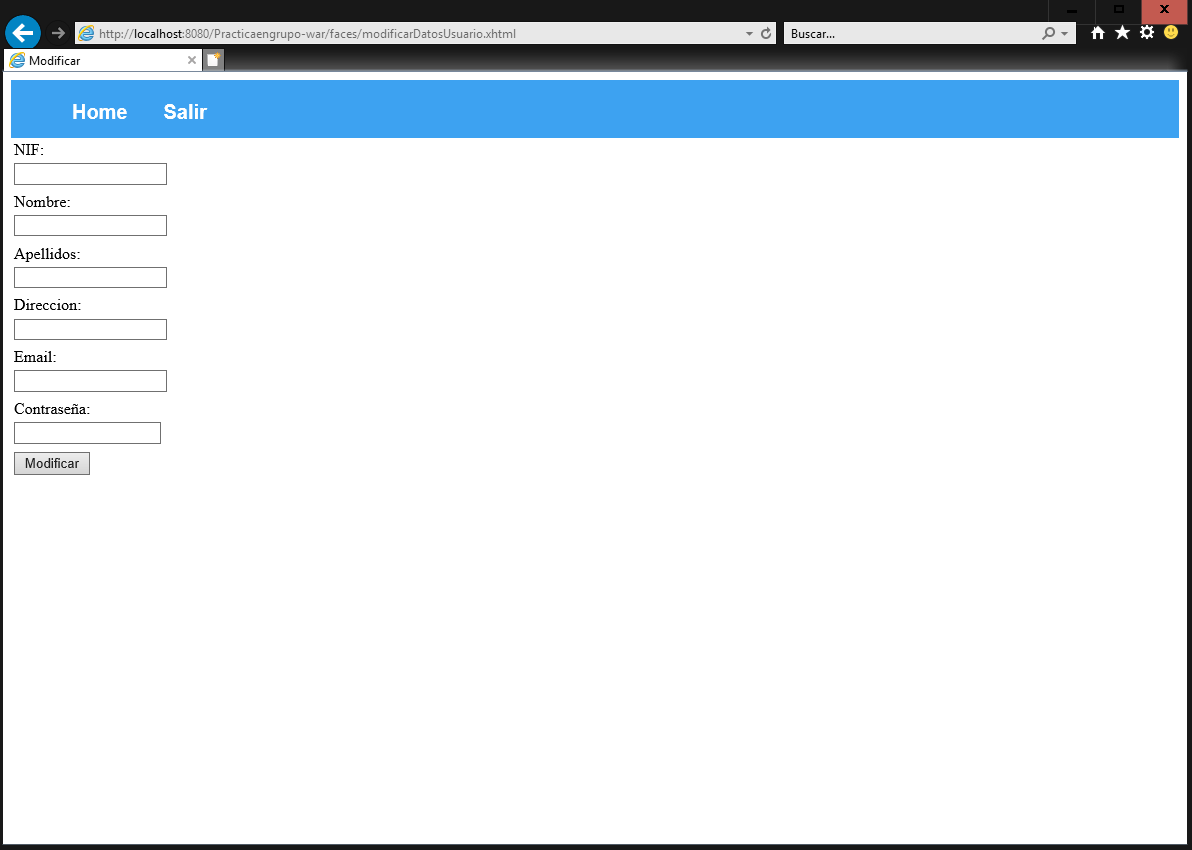
\includegraphics[scale=0.5]{capturas/MODIFICARDATOSPERSONALES.PNG}
\end{center}

\textbf{Paquete ACOES}

\begin{itemize}
\item \textbf{Control de Autorización}\\
Tenemos la variable usuario que se utiliza para llamar a la entidad Usuario de la base de datos con sus correspondientes set y get.\\
También tenemos diferentes funciones como home() que lo que hace es devolver dependiendo del rol del usuario. Si no hay usuario nos lleva a la página de "index.xhtml", si es un trabajador nos llevara a la página de "inicioTrabajador.xhtml" y si es socio a "inicioSocios.xhtml". Logout() no que hace es salir devolviendo a la página de "index.xhtml" y poniendo a usuario a null Inicio() devuelve las pagina de inicio de los usuarios
 
\item \textbf{Login}\\
Tenemos las variables negocio que nos sirve para conectar con la capa de negocio , usuario y ctrl que llama a la clase anteriormente explicada. De cada variable se encuentra sus get y set.\\
En esta clase la única función que hay es autenticar() que lo que hace es logear al usuario que introduces. Esto se hace comprobando si el usuario exite y mandándoselo al control de autorización para que nos diga a que pagina de inicio le corresponde con el rol que tiene ese usuario.
 
\item \textbf{Nino}\\
Esta clase tiene las variable negocio, nino que llama a la entidad Benficiario de la base de datos , nifBuscar que se utiliza para guarda el nif del niño que quiere ver sus datos o nota y por ultimo da que llama a la entidad Datos_Academicos con sus respectivos get y set.\\ 
Las funciones que hay son:
\begin{itemize}
\item Beneficiario(): que carga el niño que queremos ver sus datos.
\item datosAcademicos(): se encarga carga los datos académicos que queremos mostrar.
\item registrar(): te envía a la pagina "verAlumDesdeProf.xhtml" y llama a negocio para registrar al niño en la base de datos.
\item mostrarDatos(): te manda a la pagina "datosPersonalesNino.xhtml" que lo que hace es mostrar los datos del niño que para ello con el nif.
\end{itemize}
 
\item \textbf{Registro}\\
Esta clase contiene distintas variables con sus respectivos set y get.
Lo más destacable de esta clase son los siguientes procedimientos y funciones:
\begin{itemize}
\item RegistrarUsuario(): comprueba que la contraseña y su repetir sean iguales y llama al procedimiento registrarUsuario() de la capa de negocio.
\item RegistrarDonacion(): se encarga de registrar las donaciones realizadas llamando al procedimiento registrarDonacion() de la capa de negocio.
\item RegistrarNino(): registra el beneficiario del mismo modo que las funciones anteriores.
\item Apadrinar(): Se encarga de la gestión del apadrinamiento de los niños.
\item anadirCalificacion(): Su misión es añadir la calificación a los datos académicos.
\item modificarDatosUsuario(): modifica los datos del usuario activo. 
\end{itemize} 
\end{itemize}


\section{Entrega 3}

\textbf{Descripción de los EJB}\\
\textbf{AcoesException.java:} devuelve una excepción general.\\
\textbf{BeneficiarioInexistenteException.java:} devuelve una excepción al intentar buscar un niño que no pertenece a la base de datos.\\
\textbf{BeneficiarioRepetido.java:} devuelve una excepción al intentar registrar un niño que ya se encuentra en la base de datos.\\
\textbf{CalificacionRepetida.java:} devuelve una excepción al intentar añadir una calificación ya existente.\\
\textbf{ContraseniaInvalidaException.java:} devuelve una excepción al introducir una contraseña no válida.\\
\textbf{CuentaInactivaException.java:} devuelve una excepción al intentar ingresar con una cuenta no activa.\\
\textbf{CuentaInexistenteException.java:} devuelve una excepción al intentar ingresar con una cuenta inexistente.\\
\textbf{CuentaRepetidaException.java:} devuelve una excepción al intentar registrar una cuenta ya existente.\\
\textbf{Negocio.java:} interfaz que contiene los siguientes métodos:
\begin{itemize}
\item \textbf{registrarUsuario(Usuario u):} si el usuario recibido ya existe en la base de datos, devuelve una excepción. De lo contrario, lo crea.
\item \textbf{compruebaLogin(Usuario u):} comprueba que el nombre de usuario y la contraseña del usuario recibido, y que pertenecen a un usuario que existe en la BBDD. En caso contrario, devuelve una excepción.
\item \textbf{refrescarUsuario(Usuario u):} se realiza un compruebaLogin(u) y, si no devuelve una excepción, se devuelve una entidad Usuario con los datos existentes en la BBDD del usuario recibido.
\item \textbf{regisNino(Beneficiario b):} añade al niño recibido a la base de datos.
\item \textbf{refrescarNino(Beneficiario b):} se realiza un compruebaNino(b) y, si no devuelve una excepción, se devuelve una entidad Beneficiario con los datos existentes en la BBDD del niño recibido.
\item \textbf{compruebaNino(Beneficiario b):} comprueba si el niño recibido se encuentra en la base de datos. En caso contrario, devuelve una excepción.
\item \textbf{registrarDonacion(Ingresos i):} añade un nuevo ingreso.
\item \textbf{registrarCalificacion(Datos\_academicos d):} añade una nueva calificación.
\item \textbf{buscarNino(Long nif):} busca un niño en la base de datos por su NIF. Si no existe, devuelve una excepción.
\item \textbf{modificarDatosUsuario(Usuario u):} actualiza los datos de un usuario.
\item \textbf{buscarDA(Long nif):} busca los datos académicos de un niño mediante su NIF. Si no existen, devuelve una excepción.
\end{itemize}
\textbf{NegocioImpl.java:} desarrollo de los métodos definidos en Negocio.java.

\section{URL a GIT}

\href{https://github.com/LadyNightmare/ACOES}{Este} es el repositorio usado y el hash del commit es , aunque el commit posterior será con la esta memoria actualizada.

\end{document}